\documentclass[11pt,a4paper]{article}

% Define page geometry
\usepackage{geometry} \geometry{left=2.2cm, right=2.2cm, top=2.2cm, bottom=2cm}
\parskip 0.15cm 
\setlength{\parindent}{0cm} 
\usepackage{pdflscape}
\usepackage[document]{ragged2e}

% Text formatting
\usepackage[T1]{fontenc}  % Set font

\usepackage{lineno}  % Line numbers

\usepackage{amssymb}  % Symbols

\linespread{1.25}  % Linespacing

\usepackage{xcolor} \newcommand{\todo}[1]{\textcolor{red}{\textbf{#1}}}   %

% Tables
\usepackage{multirow} \setlength{\tabcolsep}{4pt}

% Image handling
\usepackage{graphicx} 

\makeatletter \g@addto@macro\@floatboxreset\centering  
\makeatother

\graphicspath{ {img/} }  % Define image path

\usepackage{subfig}  % Compound figures

\usepackage{float}  % Precise figure location

% Bibliography management
\usepackage[style=authoryear, natbib=true, backend=biber]{biblatex}
\addbibresource{lidar.bib}

% Links within document, nice figure formatting
\usepackage[breaklinks]{hyperref} \definecolor{links}{RGB}{0,0,0} \hypersetup{
	breaklinks, colorlinks=true, linkcolor=links, anchorcolor=links,
	citecolor=links, filecolor=links, menucolor=links, runcolor=links,
	urlcolor=links, pdfauthor={John L. Godlee} }
	\def\subsectionautorefname{section} \def\subsubsectionautorefname{section}

\newcommand{\beginsupplement}{% 
	\setcounter{table}{0}
	\renewcommand{\thetable}{S\arabic{table}}% 
	\setcounter{figure}{0}
	\renewcommand{\thefigure}{S\arabic{figure}}% 
}
     
% Variables

\newcommand{\titletext}{Terrestrial laser scanning}

\begin{document}

{\Large{Title: \titletext{}}}


\section*{Abstract}

\section{Introduction}

The characterization of tree canopy structure in wooded ecosystems constitutes a long-standing field of research that has been fundamental to interpreting, modelling, and improving understanding of ecosystem function \citep{Watt1947, WhittakerWoodwell1969, Horn1971}. Variation in canopy structure describes the spatial distribution and density of canopy foliage. Tree canopy foliage comprises the primary interface between trees, the atmosphere and sunlight. It is therefore essential to understand the drivers of variation in canopy structure to improve modelling efforts of earth-atmosphere carbon fluxes and community assembly \citep{}. 

At continental scales, variation in canopy height and canopy cover, two coarse measures of canopy structure both of which have been shown to affect woody productivity \citep{}, can largely be explained by climate and edaphic data \citep{SOME-GEDI}. At the scale of a single tree community however, where variation in climate and soil may be negligible, variation in canopy structure is thought to be affected principally by the tree canopy species assemblage \citep{}, and community history \citep{}. However, empirical testing of these mechanisms thought to drive canopy structure in natural wooded ecosystems remains sparse \citep{}.

Following established biodiversity-ecosystem function theory, the spatial complementarity of individual tree canopies, the niche partitioning of canopy space (hereafter `crown complementarity'), is thought to be a key mechanism underlying positive biodiversity-productivity effects in forests \citep{Pretzsch2014, Barry2019}. Biodiversity-ecosystem function theory predicts that canopy space occupation and thus canopy complexity and foliage density should increase with tree diversity, thus increasing standing biomass and woody productivity, as coexisting species must occupy non-identical niche space to avoid competitive exclusion \citep{}. 

In addition to driving variation in woody productivity and biomass, canopy structure is also expected to affect understorey biomass. A more open tree canopy which provides more light to the ground can encourage understorey growth. In mesic savannas an open tree canopy is maintained via a positive feedback where increased grassy biomass as a result of a more open canopy increases the frequency and intensity of fires which serve to maintain the open canopy \citep{}. To elucidate the tipping points which determine when savanna becomes forest, it is necessary to understand how canopy structure affects grassy biomass.

Canopy structure is multi-dimensional and has previously been explained using a plethora of metrics that originated in forest and community ecology \citep{}. Assessments of canopy structure in the dry tropical have most often modelled tree canopies as a series of ellipses (2D) or ellipsoids (3D) \citep{}. While measurements of this kind are time consuming they still present a gross oversimplification of canopy structure. Alternatively, canopy cover is often measured using indirect optical methods which partition sky from canopy material, i.e. with hemispherical photography or the commonly used LAI-2000, providing a 2D representation of the canopy that is a simplification in other ways. In recent years, particularly in temperate and boreal forests, LiDAR (Light Detection And Ranging) has emerged as a suitable technology for rapidly and precisely assessing canopy structure in 3D, while conserving the complexity of the canopy. Applications of LiDAR can be classified into three principal groups based on the spatial resolution of the resulting data. In order from lowest to highest spatial resolution: 1) satellite LiDAR, 2) airborne LiDAR, and 3) terrestrial LiDAR.

In this study we applied terrestrial LiDAR techniques to mesic savannas at two sites in southern Africa, with the aim of increasing our understanding of how tree canopy structure is affected by tree neighbourhood composition and stand structure. We also investigated how this variation in canopy structure affects understorey grassy biomass. 

\section{Materials and methods}

\subsection{Study sites}

Measurements were conducted at two sites, the first in Bicuar National Park, southwest Angola (S15.1$^\circ$, E14.8$^\circ$), and the second in Kilwa District, southeast Tanzania (S9.0$^\circ$, E39.0$^\circ$) (\autoref{map}).

\begin{figure}[H]
\centering
	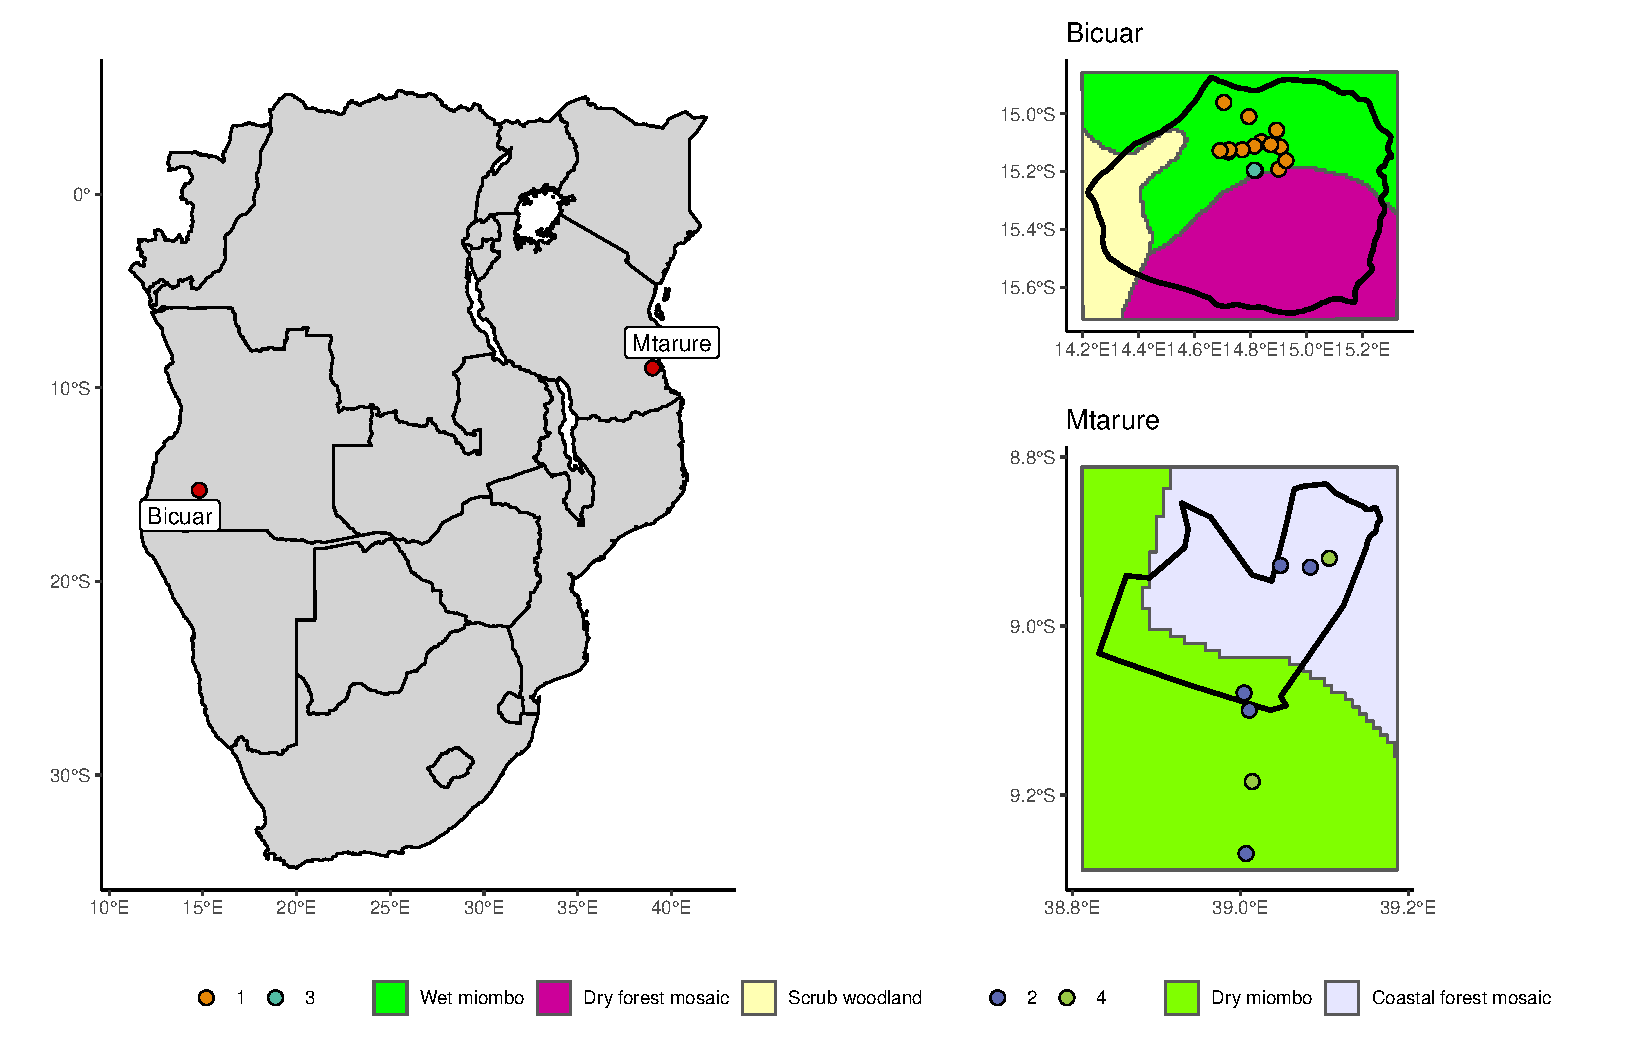
\includegraphics[width=\textwidth]{map}
	\caption{Location of study sites within southern Africa (a), and of 1 ha plots within each site. The blue polygons denote the boundaries of protected areas which encompass the majority of study sites, Bicuar National Park in Angola (b), and Mtarure Forest Reserve in Tanzania (c).}
	\label{map}
\end{figure}

\subsection{Field measurements}

Fieldwork was conducted between February and April at both sites, during the peak growth period of each site, in order to capture the highest leafy volume in the canopy and the largest grassy volume in the understorey.

At each site, 1 ha permanent plots were sampled. In Angola, 15 plots were sampled, while in Tanzania, seven were sampled, following the curtailment of fieldwork due to COVID-19 travel restrictions.

Each permanent plot was further subdivided into nine 10 m diameter circular subplots arranged in a regular grid, with a buffer from the plot edge (\autoref{subplot}).

\begin{figure}[H]
\centering
	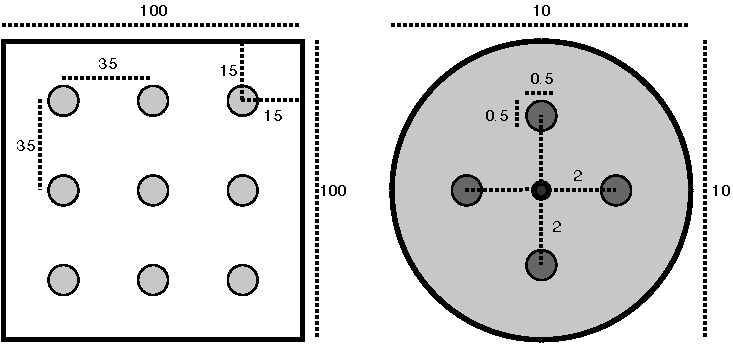
\includegraphics[width=\textwidth]{subplot}
	\caption{The layout of 10 m diameter subplots within each 1 ha square plot. Each subplot is situated inside a 15 m buffer from the plot edge, with 35 m between subplot centres. Subplots are arranged in a 3x3 grid. Disc-pasture measurements and biomass samples are located in cardinal directions 2 m from the centre of the subplot. All distances are in metres.}
	\label{subplot}
\end{figure}

For each subplot, we measured all woody stems >5 cm trunk diameter with canopy material inside the subplot. We identified each stem to species and measured trunk diameter (diameter at breast height - 1.3 m), height to top of canopy material, canopy area calculated as an ellipse of two perpendicular crown diameter measurements, distance and direction from subplot centre.

At the centre of each subplot a photograph was taken with a Nikon D750 full-frame DSLR camera, with a Sigma 8 mm f/3.5 EX DG circular fisheye lens. This lens has an equisolid (equal area) projection, which avoids image distortion. The photo was taken facing directly to zenith, with the top of the camera facing to magnetic north, at a height of 1.3 m or above understorey vegetation, whichever was higher. Photos were captured under uniform light conditions as much as possible, either under overcast skies or early in the day before direct sunlight could be seen on the photo. 

\subsection{Terrestrial laser scanning}

Within each subplot, a variable number of scans were recorded using a Leica HDS6100 phase-shift terrestrial laser scanner (TLS). The number and position of scans within a subplot was determined by the arrangement and density of canopy material in the subplot. Scan positions were arranged to minimise shadows within the canopy, and to maximise canopy penetration. Number of scans per subplot ranged between one and five in both Angola and Tanzania (\autoref{scan_settings}).


\subsection{Data analysis}

Registration of multiple scans from different locations allows us to minimise the occlusion effect and improve canopy penetration.

\subsubsection{Scan processing}

Point clouds from scans in each subplot were registered and unified using Leica Cyclone (version 9.1). Targets from each scan were aligned using Cyclone's automatic target acquisition. 

Voxelisation: Points don't have an area or defined volume and so are unsuitable for estimating hemispherical points \citep{Seidel2012}.

Partial interceptions with phase-shift laser scanners can produce erroneous results and must be accounted for. I did this by removing noise from the point cloud.


Objects located closer to the instrument will be represented by a higher density of points, resulting in an imbalanced representation of the measured 3D space.

Resultant points clouds had ~points, ~points after filtering, ~voxels after voxelisation.

Classified ground points using the Progressive Morphological Filter (PMF) from \citep{Zhang2003}. Reclassified height based on this revised ground layer by measuring the vertical distance between the nearest ground point and each point.

We used ray-tracing (POV-ray) to calculate gap fraction from TLS scans at the centre of each subplot. Voxels were converted to cubes filling the voxel volume, with a ``camera'' placed at the subplot centre at 1.8 m height, at a height of 1.8 m. Used a fisheye lens with a view angle of 180 degrees, with matt black Cubes against a white background and no light source. The images produced by POV-ray were analysed using Hemiphot in an identical manner to the hemispherical photographs.

\section{Results}

\section{Discussion}

\section{Conclusion}

\printbibliography

\section{Supplementary Material} \beginsupplement

\end{document}
